Let the boundary of the EB be given by ($a>b>0$):
\begin{equation}
f(x,y)=\left(\frac{x}{a}\right)^2+\left(\frac{y}{b}\right)^2=1.
\label{eqn:billiard-f}
\end{equation}

We describe a numerically-assisted method\footnote{We started with visual inspection, but this is both laborious and unreliable, some loci (take $X_{30}$ and $X_6$ as examples) are indistinguishable from ellipses to the naked eye.} which proves that the locus of a given Triangular Center is elliptic or otherwise. We then apply it to the first 100 Triangle Centers\footnote{An arbitrarily large list can be tested.} listed in \cite{etc}.

\subsection{Proof Method}

Our proof method consists of two phases, one numeric, and one symbolic, Figure~\ref{fig:method-pipeline}. It makes use of the following Lemmas, whose proofs appear in Appendix~\ref{app:method-lemmas}:

\begin{lemma}
The locus of a Triangle Center $X_i$ is symmetric about both EB axes and centered on the latter's origin.
\label{lem:axisymmetric}
\end{lemma}

\begin{proof} 
Given a 3-periodic $T=P_1P_2P_3$. Since the EB is symmetric about its axes, the family will contain the reflection of $T$ about said axes, call these $T'$ and $T''$. Since Triangle Centers are invariant with respect to reflections, Appendix~\ref{app:triangle-centers}, $X_i'$ and $X_i''$ will be found at similary reflected locations.
\end{proof}

Note that  if the locus is elliptic, the above implies it will be concentric and axis-aligned with the EB.

%\begin{lemma}
%\label{lem:axisymmetric}
%The locus of a Triangle Center $X_i$ is symmetric about both EB axes and centered on the latter's origin.
%\end{lemma}

%\begin{proof} Let $X_i =(c_i,d_i)$ be a triangular center of the billiard orbit $P_1=(x_1,y_1), P_2=(x_2,y_2), P_3=(x_3,y_3)$. For the reflections $\pi_1(x,y)=(x,-y)$,   $\pi_2(x,y)=(-x,y)$ and antipodal $\pi_3(x,y)=-(x,y)$ the triangles $Q_1=\pi_j(P_1), Q_2=\pi_j(P_2), Q_3=\pi_j(P_3)$, ($j=1,2,3$), are also   billiard orbits, and by equation \eqref{eqn:trilin-cartesian} its triangular center is $Y_i=\pi_j(X_i). $  This ends the proof.
%
%\end{proof}

\begin{lemma}
\label{lem:axis-of-symmetry}
Any Triangle Center $X_i$ of an isosceles triangle is on the axis of symmetry of said triangle.
\end{lemma}

\begin{lemma}
\label{lem:center-cover}
A parametric traversal of $P_1$ around the EB boundary triple covers the locus of Triangle Center $X_i$, elliptic or not.
\end{lemma}

See Section~\ref{sec:triple-winding} for more details.

A first phase fits a concentric, axis-aligned ellipse to a fine sampling of the locus of some Triangle Center $X_i$. A good fit occurs when the error is several orders of magnitude\footnote{Robust fitting of ellipses to a cloud of points is not new \cite{fitzgibbon99-ellipse}. In our case, the only source of error in Triangle Center coordinates is numerical precision, whose propagation can be bounded by Interval Analysis \cite{moore2009-interval-analysis,snyder92-ellipse}.} less than the sum of axes regressed by the process. False negatives are eliminated by setting the error threshold to numeric precision. False positives can be produced by adding arbitrarily small noise to samples of a perfect ellipse, though this type of misclassification does not survive the next, symbolic phase. 

A second phase attempts to symbolically verify via a Computer Algebra System (CAS) if the parametric locus of the $X_i$ satisfies the equation of a concentric, axis-aligned ellipse. Expressions for its semi-axes are obtained by evaluating $X_i$ at isosceles orbit configurations, Figure~\ref{fig:sideways-upright-orbit}. The method is explained in detail in Figure~\ref{fig:method-detail}.

\begin{figure}
    \centering
    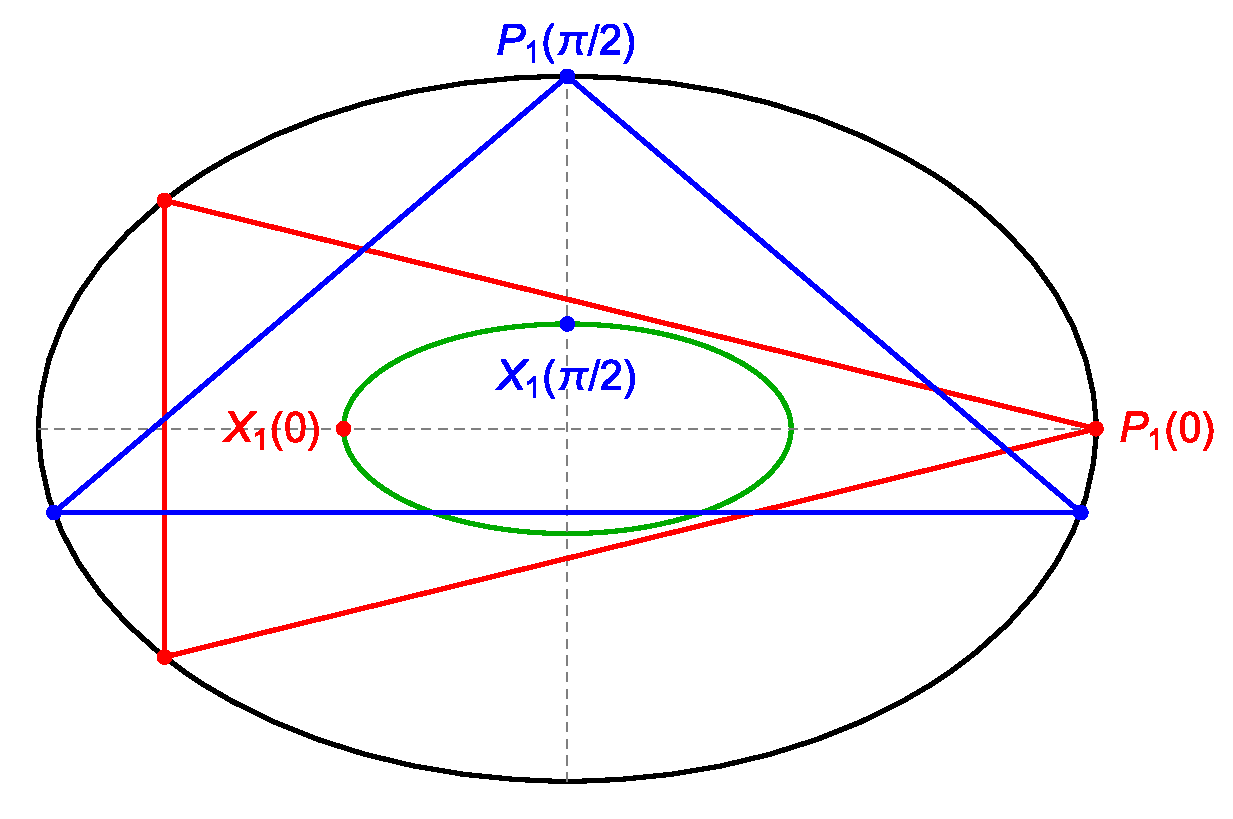
\includegraphics[width=.5\textwidth]{pics_1060_two_isosceles}
    \caption{With $P_1$ at the right (resp.~top) vertex of the EB, the orbit is a sideways (resp.~upright) isosceles triangle, solid red (resp.~solid blue). Not shown are their two symmetric reflections. Also shown (green) is the locus of a sample Triangle Center, $X_1$ in this case. At the isosceles positions, vertices will lie on the axis of symmetry of the triangle, Lemma~\ref{lem:axis-of-symmetry}. When the locus is elliptic, the $x,y$ coordinates of $X_i(0),X_i(\pi/2)$ are the semi-axes $a_i,b_i$, respectively.}
    \label{fig:sideways-upright-orbit}
\end{figure}

\begin{figure}
    \centering
    %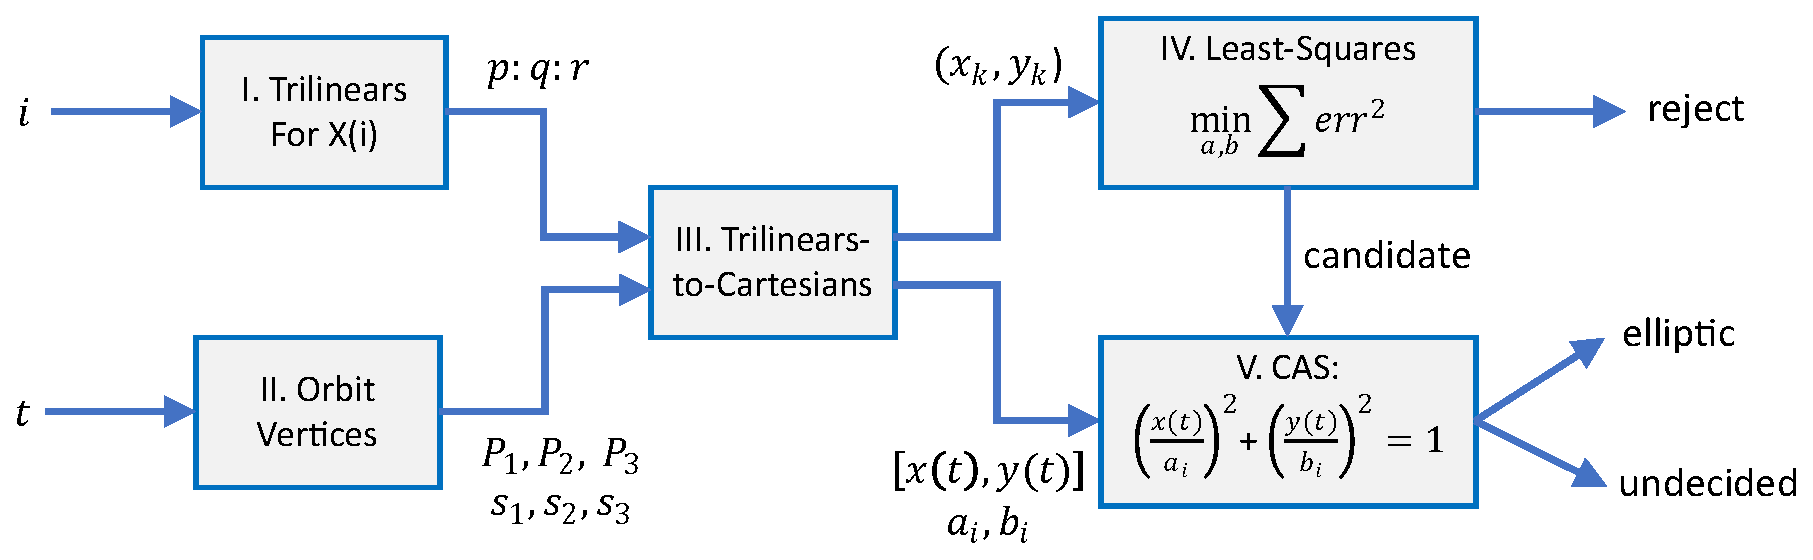
\includegraphics[trim={0 7.5cm 0 1cm},clip,width=\textwidth]{pics_1130_algo_proof_elliptic.eps}
    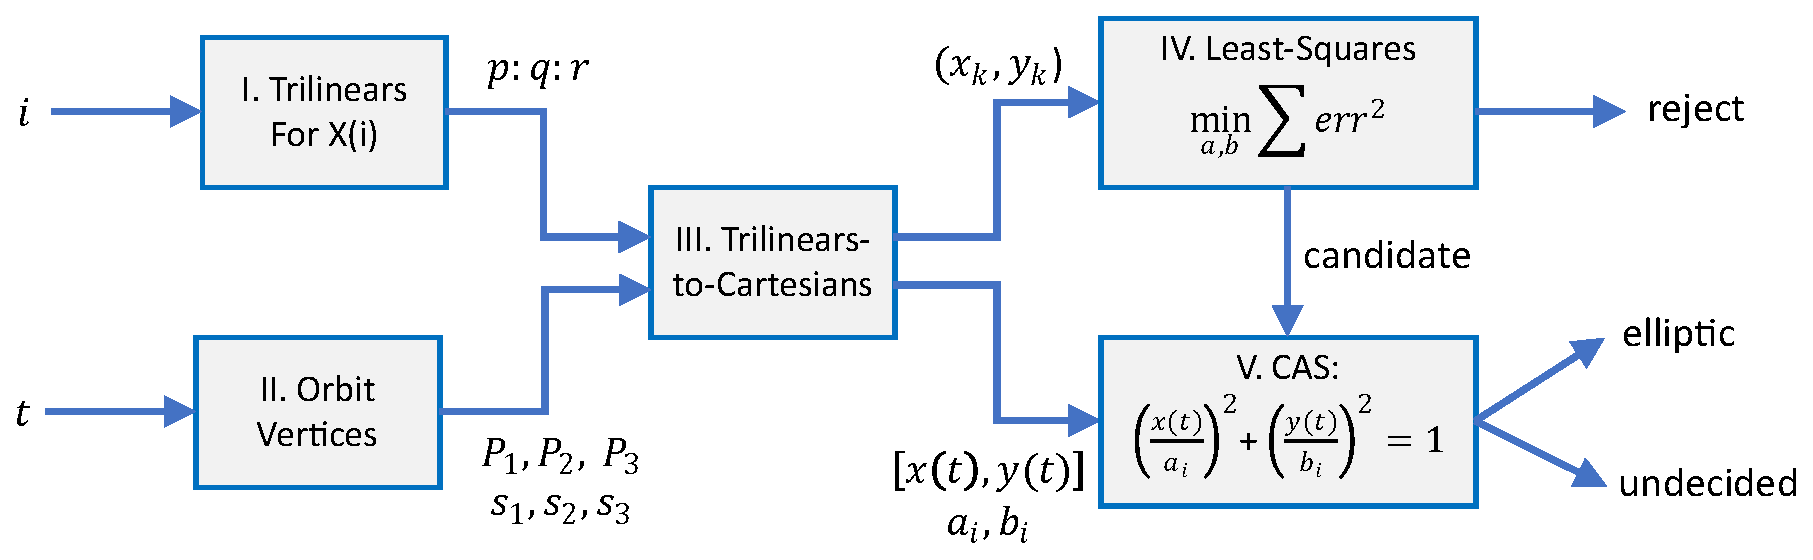
\includegraphics[width=.9\textwidth]{pics_1130_algo_proof_elliptic.eps}
    \caption{Our method as a flow-chart, modules labeled from I to V: (I) The ith center is specified and its Trilinears $p:q:r$ are obtained from ETC \cite{etc}. (II) Given a symbolic parameter $t$ or a numeric sample $t_k$, obtain Cartesians for orbit vertices and the sidelengths, Appendix~\ref{app:p1p2p3}. (III) Combine Trilinears and orbit data to obtain, via \eqref{eqn:trilin-cartesian}, numeric Cartesians for $X_i(t_k)$ or symbolically as $X_i(t)$. (IV) Least-squares fit an axis-aligned, concentric ellipse to the $(x_k,y_k)$ samples and accept $X_i$ as candidate if the fit error is sufficiently small. (V) Verify, via a Computer Algebra System (CAS), if the parametric locus $X_i(t)$ satisfies the equation of an ellipse whose axes $a_i,b_i$ are obtained symbolically in II-III by setting $t=0,\pi/2$. If the CAS is successful, $X_i(t)$ is deemed elliptic, otherwise the result is ``undecided''. The CAS was successful for all 29 candidates selected by IV out of the first 100 Kimberling Centers.}
    \label{fig:method-pipeline}
\end{figure}

% The philosophy: 

%In the quest to determine  elliptic loci, an human observer could discard, visually,  plots having loops and/or that are non convex.  However, it could be quite a different story   to distinguish a (true)  ellipse from a symmetric oval, just visually, as the plots of   $X_6$  and $X_?$ exemplify.   This  task is outside our realm - it may belong to neuroperception. Architects and painters do have a keen eye but even so there is a limit to their abilities \cite{Ochkov2019}, \cite{Xing2018}, \cite{Duvernoy2015}, \cite{Mazzotti2017}. 

%Hence we  opted to avoid   direct human involvement. The ideia is to  work  as much as possible in an automated fashion.  

%Pattern recognition algorithms for ellido exist, but they are costly. Moreover, we feared %that could be  prone to false positives or negatives. 

%The screening procedure:

% \subsection{Outline of the two steps}
\begin{figure}
\fbox{
\begin{minipage}{\textwidth}
\footnotesize
\noindent \textbf{1. Select Candidates:}
\begin{itemize}
\item Let the EB have axes $a,b$ such that $a>b>0$. Calculate $P_1(t_k)=\left(a\cos(t_k),b\sin(t_k)\right)$, for $M$ equally-spaced samples $t_k\in[0,2\pi)$, $k=1,2,...,M$.
\item Obtain the Cartesian coordinates for the orbit vertices $P_2(t_k)$ and $P_3(t_k)$, $\forall k$ (Appendix~\ref{app:p1p2p3}).
\item Obtain the Cartesians for Triangle Center $X_i$ from its Trilinears \eqref{eqn:trilin-cartesian}, for $\forall{t_k}$. If analyzing the vertex of a Derived Triangle, convert a row of its {\em Trilinear Matrix} to Cartesians, Appendix~\ref{app:derived-tris}.
\item Least-squares fit an origin-centered, axis-aligned ellipse (2 parameters) to the $X_i(t_k)$ samples, Lemma~\ref{lem:axisymmetric}. Accept the locus as potentially elliptic if the numeric fit error is negligible, rejecting it otherwise.
\end{itemize}
\noindent \textbf{2. Verify with CAS}
\begin{itemize}
    \item Taking $a,b$ as symbolic variables, calculate $X_i(0)$ (resp.~$X(\pi/2)$), placing $P_1$ at the right (resp.~top) EB vertex. The orbit will be a sideways (resp.~upright) isosceles triangle, Figure~\ref{fig:sideways-upright-orbit}. By Lemma~\ref{lem:axis-of-symmetry}, $X_i$ will fall along the axis of symmetry of either isosceles.
    \item The $x$ coordinate of $X_i(0)$ (resp.~the $y$ of  $X_i(\pi/2)$) will be symbolic expressions in $a,b$. Use them as candidate locus semiaxes' lengths $a_i,b_i$.
    \item Taking $t$ as a symbolic variable, use a computer algebra system (CAS) to verify if $X_i(t)=\left(x_i(t),y_i(t)\right)$, as parametrics on $t$, satisfy $(x_i(t)/a_i)^2+(y_i(t)/b_i)^2=1$, ${\forall}t$.
    \item If the CAS is successful, Lemma~\ref{lem:center-cover} guarantees $X_i(t)$ is will cover the entire ellipse, so assert that the locus of $X_i$ is an ellipse. Else, locus ellipticity is indeterminate. 
\end{itemize}
\end{minipage}}
\caption{Method for detecting ellipticity of a Triangle Center locus.}
\label{fig:method-detail}
\end{figure}

\subsection{Phase 1: Least-Squares-Based Candidate Selection}

Let the position of $X_i(t)$ be sampled\footnote{Randomly or in equal intervals.} at $t_k\in[0,2\pi]$, $k=1{\ldots}M$. If the locus is an ellipse, than the latter is concentric and axis-aligned with the EB, Lemma~\ref{lem:axisymmetric}. Express the squared error as the sum of squared sample deviations from an implicit ellipse:

\begin{equation}
\text{err}^2(a_i,b_i)= \sum_{k=1}^M{\left[\left(\frac{x_k}{a_i}\right)^2+\left(\frac{y_k}{b_i}\right)^2-1\right]^2}
\label{eqn:fit-error}
\end{equation}

\noindent Least-squares can be used to estimate the semi-axes:

$$
(\hat{a_i},\hat{b_i})=\argmin_{a,b}\left\{ \text{err}^2(a_i,b_i)\right\}
$$

The first 100 Kimberling centers separate into two distinct clusters: 29 with negligible least-squares error, and 71 with finite ones. These are shown in ascending order of error in our companion website \cite[Part II]{garcia2021-ellipses-web}.

A gallery of loci generated by $X_1$ to $X_{100}$ (as well as vertices of several derived triangles) is provided in \cite{dsr_locus_gallery_2019}.

\subsection{Phase 2: Symbolic Verification with a CAS}

A CAS was successful in symbolically verifying that all 29 candidates selected in Phase 1 satisfy the equation of an ellipse (none were undecided). As an intermediate step, explicit expressions for their elliptic semi-axes were computed and appear in \cite[Part I]{garcia2021-ellipses-web}.

\begin{theorem} \label{main}
Out of the first 100 centers in \cite{etc}, exactly 29 produce elliptic loci, all of which are concentric and axis-aligned with the EB. These are $X_i$,i=1, 2, 3, 4, 5, 7, 8, 10, 11, 12, 20, 21, 35, 36, 40, 46, 55, 57, 63, 65, 72, 78, 79, 80, 84, 88, 90. Specifically:
\begin{itemize}
\item The loci of $X_i,i=2,7,57,63$ are ellipses similar to the EB.
\item The loci of $X_i,i=4,10,40$ are ellipses similar to a $90^\circ$-rotated copy of the EB.
\item The loci of $X_i,i=88,100$ are ellipses identical to the EB\footnote{See below for more centers on the EB discovered by Peter Moses and Deko Dekov.}.
\item The loci of $X_{55}$ is an ellipse similar to the $N=3$ Caustic.
\item The loci of $X_i,i=3,84$ are ellipses similar to a $90^\circ$-rotated copy of the $N=3$ Caustic.
\item The locus of $X_{11}$ is an ellipse identical to the $N=3$ Caustic.
\end{itemize}
\label{thm:loci29}
\end{theorem}

The properties above are summarized on Table~\ref{tab:ell}. Explicit expressions for the semi-axes in terms of $a,b$ for the above appear in \cite[Part I]{garcia2021-ellipses-web}. 

\begin{figure}
    \centering
    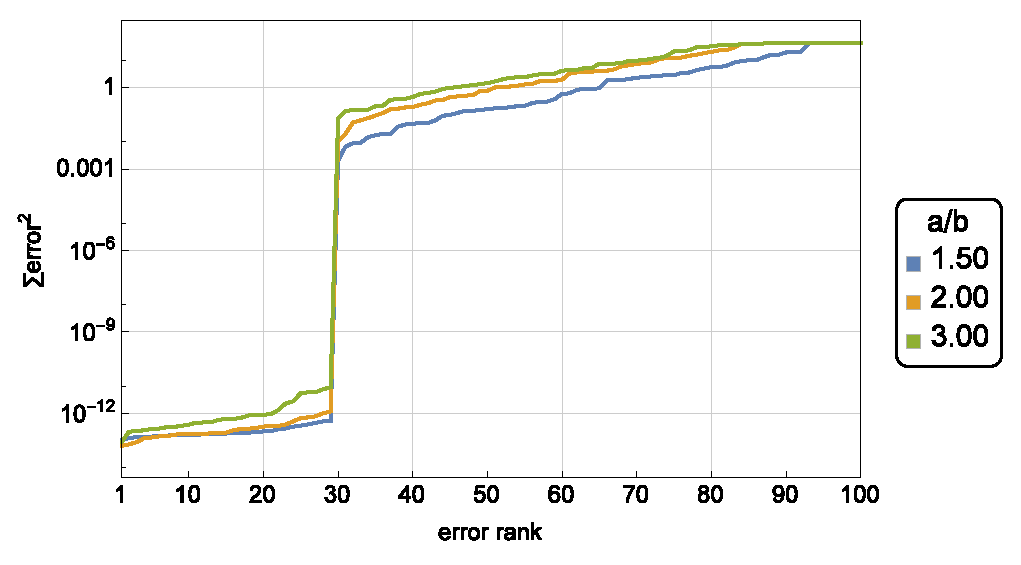
\includegraphics[width=.7\textwidth]{pics_1100_least_squares_error.eps}
    \caption{Log of Least-squares error for first 100 Kimberling centers in ascending order of error, for three values of $a/b$, $M=1500$. Elliptic vs. non-elliptic centers are clearly separated in two groups whose errors differ by several orders of magnitude. A table in \cite[Part II]{garcia2021-ellipses-web} shows that $X_{37}$ and $X_6$ are have ranks $30$ and $31$ respectively, i.e., they are the Centers whose non-elliptic loci are closest to a perfect ellipse.}
    \label{fig:least-squares-error-graph}
\end{figure}

\begin{table}
%\renewcommand{\arraystretch}{1.}
\begin{minipage}[t]{.475\linewidth}
$$
\scriptsize
\begin{array}{|c|c|l|c|}
\hline
\text{row} & X_i & \text{definition} & \text{sim} \\
\hline
 1 & {1} & \text{Incenter} & \text{J}^t \\
 2 & {2} & \text{Centroid} & \text{B} \\
 3 & {3} & \text{Circumcenter} & \text{C}^t  \\
 4 & {4} & \text{Orthocenter} & \text{B}^t \\
 5 & {5} & \text{9-Point Center} &  \\
 6 & {7} & \text{Gergonne Point} & \text{B}\\
 7 & {8} & \text{Nagel Point} &  \\
 8 & {10} & \text{Spieker Center} & \text{B}^t\\
 9 & {11} & \text{Feuerbach Point} & \text{C}^+ \\
 10 & {12} & \text{$\{X_{1,5}\}$-Harm.Conj. of $X_{11}$} & \\
 11 & {20} & \text{de Longchamps Point} & \\
 12 & {21} & \text{Schiffler Point} & \\
 13 & {35} & \text{$\{X_{1,3}\}$-Harm.Conj. of $X_{36}$} & \\
 14 & {36} & \text{Inverse-in-Circumc. of $X_1$} & \\
 15 & {40} & \text{Bevan Point} & \text{B}^t \\
 \hline
\end{array}
$$
\end{minipage}%
\begin{minipage}[t]{.475\linewidth}
$$
\scriptsize
\begin{array}{|c|c|l|c|}
\hline
\text{row} & X_i & \text{definition} & \text{sim} \\
\hline
16 & {46} & \text{$X_4$-Ceva Conj. of $X_1$} & \\
 17 & {55} & \text{Insimilictr(Circumc.,Incir.)} & \text{C}\\
 18 & {56} & \text{Exsimilictr(Circumc.,Incir.)} &  \\
 19 & {57} & \text{Isogonal Conj. of $X_9$} & \text{B} \\
 20 & {63} & \text{Isogonal Conj. of $X_{19}$} & \text{B} \\
 21 & {65} & \text{Intouch Triangle's $X_4$} & \\
 22 & {72} & \text{Isogonal Conj. of $X_{28}$} & \text{J}\\
 23 & {78} & \text{Isogonal Conj. of $X_{34}$} & \\
 24 & {79} & \text{Isogonal Conj. of $X_{35}$} & \\
 25 & {80} & \text{Refl. of $X_1$ about $X_{11}$} &  \text{J}^t \\
 26 & {84} & \text{Isogonal Conj. of $X_{40}$} & C^t \\
 27 & {88} & \text{Isogonal Conj. of $X_{44}$} &  \text{B}^+ \\
 28 & {90} & \text{$X_{3}$-Cross Conj. of $X_{1}$} & \\
 29 & {100} & \text{Anticomplement of $X_{11}$} & \text{B}^+\\
 \hline
 \end{array}
 $$
\end{minipage}
\caption{The 29 Kimberling centers within $X_1$ to $X_{100}$ with elliptic loci. Under column ``sim.'', letters B,C,J indicate the locus is similar to EB, Caustic, or Excentral locus, respectively. An additional {+}  (resp. {t}) exponent indicates the locus is identical (resp. similar to a perpendicular copy) to the indicated ellipse. Note: the ellipticity of  $X_i$,$i=1,2,3,4$ was previously proven \cite{olga14,sergei2016proj,corentin19,garcia2019-incenter}.}
\label{tab:ell}
\end{table}

\subsection{The quartic locus of the Symmedian Point}
\label{sec:symmedian}

At $a/b=1.5$ the locus of $X_6$, the Symmedian Point, is visually indistinguishable from an ellipse, Figure~\ref{fig:symmedian}. Fortunately, its fit error is 10 orders of magnitude higher than the ones produced by true elliptic loci, see \cite[Part II]{garcia2021-ellipses-web}. So it is easily rejected by the least-squares phase. Indeed, symbolic manipulation yields:

\begin{theorem}
 The locus of $X_6$ is a convex quartic given by:

\begin{equation*}
  \mathcal{X}_6(x,y)=c_1 x^4+c_2 y^4+c_3 x^2 y^2+ c_4 x^2 + c_5 y^2 = 0
\end{equation*}

\noindent where:
$$
\begin{array}{rlrl}
c_1=&b^4(5\delta^2-4(a^2-b^2)\delta -a^2 b^2)&c_2=&a^4(5\delta^2+4(a^2-b^2)\delta-a^2b^2) \\
c_3=&2a^2 b^2(a^2 b^2+3\delta^2)&c_4=&a^2 b^4(3 b^4+2(2 a^2-b^2)\delta-5\delta^2)\\
c_5=&a^4 b^2(3 a^4+2(2 b^2-a^2)\delta-5\delta^2)&\delta=&\sqrt{a^4-a^2 b^2+b^4}
\end{array}
$$
\end{theorem}

\begin{proof}
Using a CAS, obtain symbolic expressions for the coefficients of a quartic symmetric about both axes (no odd-degree terms), passing through 5 known-points. Still using a CAS, verify the symbolic parametric for the locus satisfies the quartic.
\end{proof}

 \noindent Note the above is also satisfied by a degenerate level curve $(x,y)=(0,0)$, which we ignore.

\begin{remark}
The axis-aligned ellipse $\mathcal{E}_6$ with semi-axes $a_6,b_6$ is internally tangent to $\mathcal{X}_6(x,y)=0$ at the four vertices where:
{\small  
\begin{align}
%a_6=&\frac{\left[(3\,a^2-b^2)\delta %-(a^2+b^2)b^2\right]a}{a^4+b^4+2\delta^2}\nonumber\\
a_6= \frac{\left[(3\,a^2-b^2)\delta -(a^2+b^2)b^2\right]a}{a^2b^2+3\delta^2},\;\;\;
b_6= \frac{\left[(a^2-3\,b^2)\delta + (a^2+b^2)a^2\right]b}{a^2b^2+3\delta^2}
\label{eqn:x6-ellipse}
\end{align}
}
\end{remark}

\begin{figure}
    \centering
    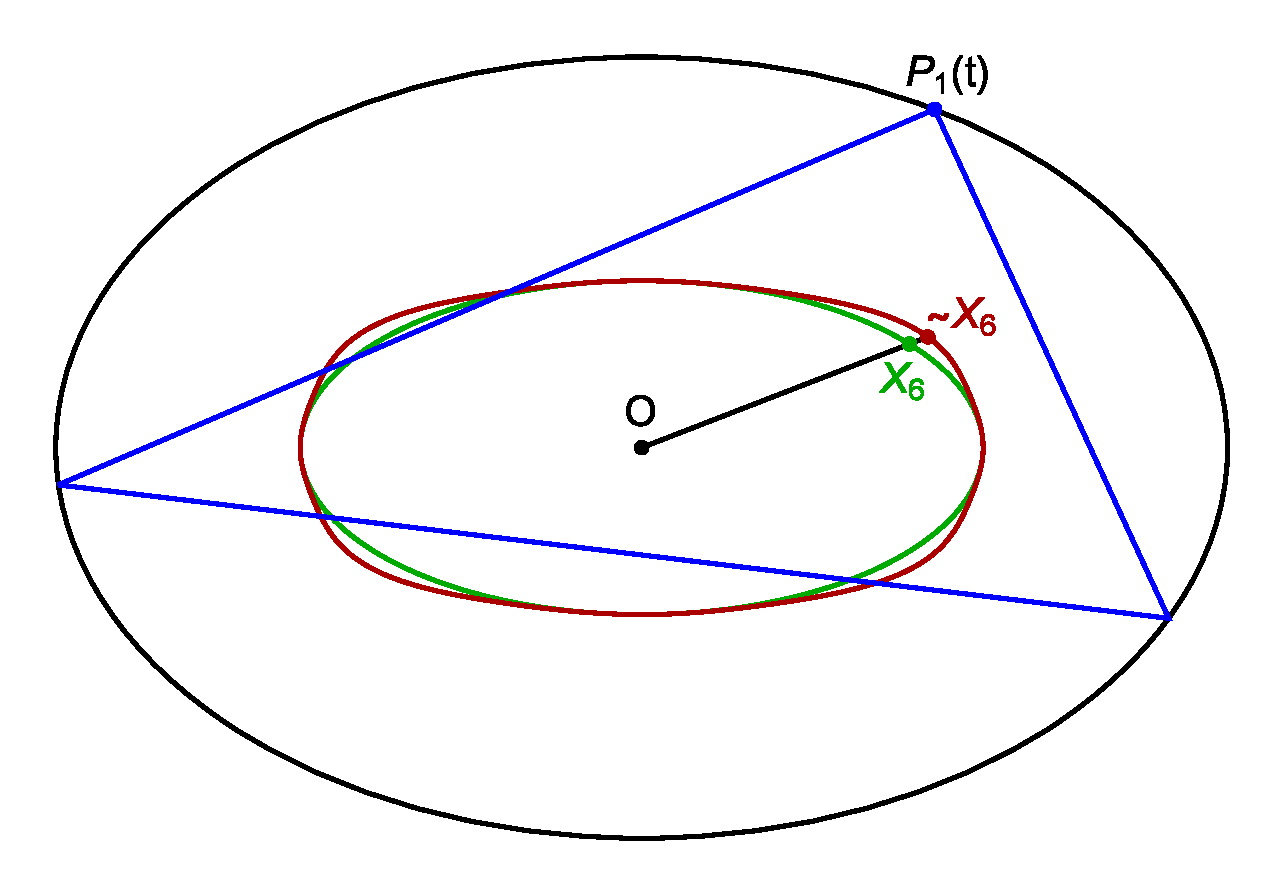
\includegraphics[width=.6\textwidth]{pics_1110_symmedian.eps}
    \caption{An $a/b=1.5$ EB is shown (black) as well as a sample 3-periodic (blue). At this aspect ratio, the locus of $X_6$ (green) is indistinguishable to the naked eye from a perfect ellipse. To see it is non-elliptic, consider the locus of a point ${\sim}X_6(t)=X_6(t)+k|X_6(t)-Y_6'(t)|$, with $k=2{\times}10^6$ and $Y_6'(t)$ the intersection of $OX_6(t)$ with a best-fit ellipse (visually indistinguishable from green), \eqref{eqn:x6-ellipse}. \href{https://bit.ly/3qc0Z0L}{app}}
    \label{fig:symmedian}
\end{figure}

Table~\ref{tab:quartic-coeffs} shows the above coefficients numerically for a few values of $a/b$.

\begin{table}[H]
    \centering
$$
\begin{array}{|c|c|c|c|c|c|c|c|}
\hline
 \text{a/b} & a_6 & b_6 & c_1/c_3 & c_2/c_3 & c_4/c_3 & c_5/c_3 & A(\mathcal{E}_6)/A(\mathcal{X}_6) \\
 \hline
  1.25 & 0.433 & 0.282 & 0.211 & 1.185 & -0.040 & -0.095 & 0.9999 \\
 1.50 & 0.874 & 0.427 & 0.114 & 2.184 & -0.087 & -0.399 & 0.9998 \\
 2.00 & 1.612 & 0.549 & 0.052 & 4.850 & -0.134 & -1.461 & 0.9983 \\
 3.00 & 2.791 & 0.620 & 0.020 & 12.423 & -0.157 & -4.769 & 0.9949 \\
 \hline
\end{array}
$$
\caption{Coefficients $c_i/c_3$, $i=1,2,4,5$ for the quartic locus of $X_6$ as well as the axes $a_6,b_6$ for the best-fit ellipse, for various values of $a/b$. The last-column reports the area ratio of the internal ellipse $\mathcal{E}_6$ (with axes $a_6,b_6$) to that of the quartic locus $\mathcal{X}_6$, showing an almost exact match.}
\label{tab:quartic-coeffs}
\end{table}

\subsection{Locus Triple Winding}
\label{sec:triple-winding}

As an illustration of Lemma~\ref{lem:center-cover}, consider the elliptic locus of $X_1$, the Incenter\footnote{The same argument is valid for the non-elliptic locus of, e.g., $X_{59}$, Figure~\ref{fig:incenter-loci} (right).}. Consider the locus of a point $Y_1$ located on between $X_1$ and an Intouchpoint $I_1$, Figure~\ref{fig:incenter-loci} (left):
 
\begin{equation*}
Y_1(t;\rho)=(1-{\rho})X_1(t)+{\rho}I_1(t),\;\;\;\rho\in[0,1]
 \end{equation*}
 
\noindent When $\rho=1$ (resp. $0$), $Y_1(t)$ is the two-lobe locus of the Intouchpoints (resp. the elliptic locus of $X_1$). With $\rho$ just above zero, $Y_1$ winds thrice around the EB center. At $\rho=0$, the two lobes and the remainder of the locus become one and the same: $Y_1$ winds thrice over the locus of the Incenter, i.e., the latter is the limit of such a convex combination.

It can be shown that at $\rho=\rho^*$, with $\rho^*=1-(b/a)^2$, the two $Y_1(t)$ lobes touch at the the EB center. When $\rho>\rho^*$ (resp. $\rho<\rho^*$), the locus of $Y_1(t)$ has winding number 1 (resp. 3) with respect to the EB center, see Figure~\ref{fig:inc-wind3}.

A similar phenomenon occurs for loci of convex combinations of the following pairs: (i) Barycenter $X_2$ and a side midpoint, (ii) Circumcenter $X_3$ and a side midpoint, (iii) Orthocenter $X_4$ and altitude foot, etc., see \cite[pl\#11,12]{dsr_playlist_2020}.

\begin{figure}
    \centering
    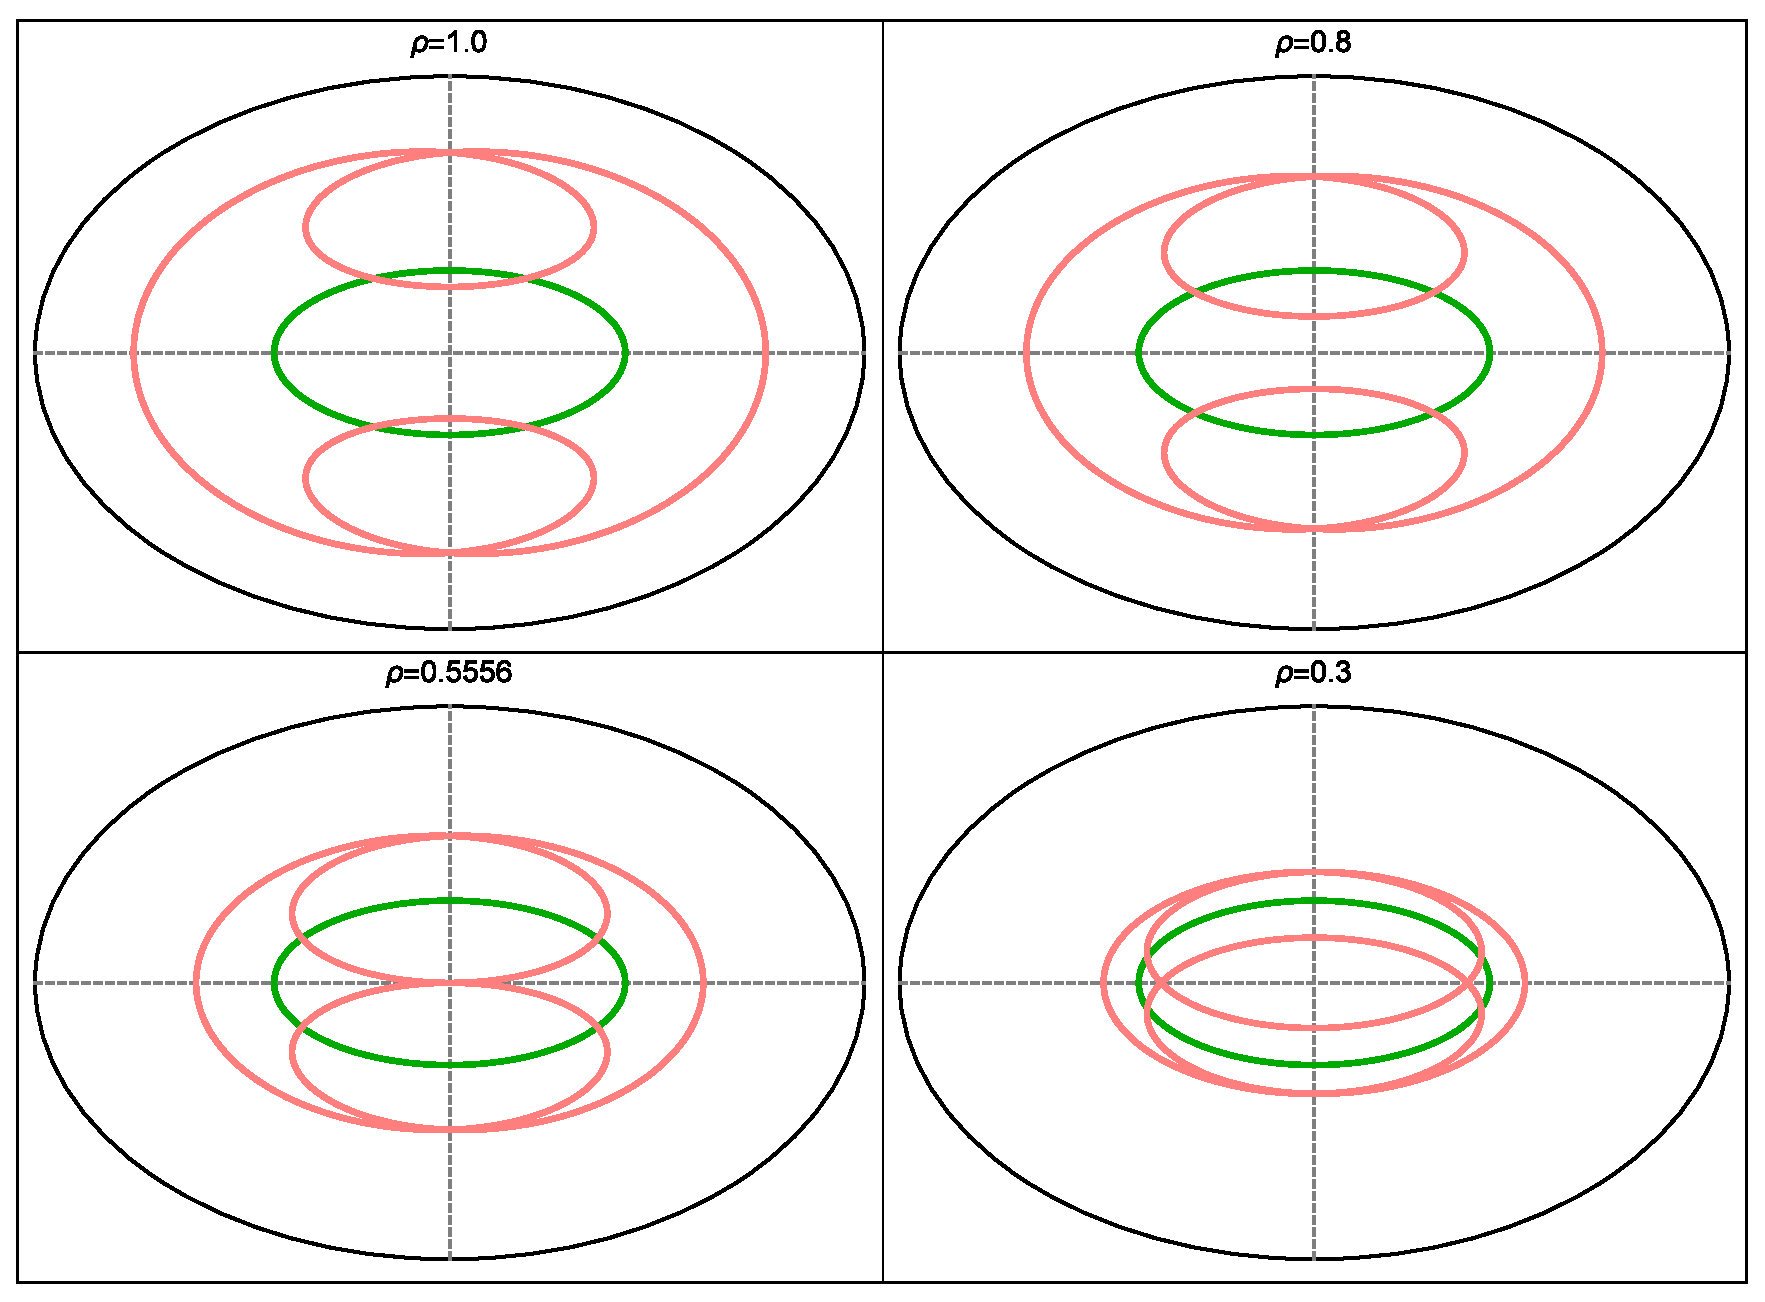
\includegraphics[width=\textwidth]{pics_1090_conv_inc_pedal.eps}
    \caption{An $a/b=1.5$ EB is shown (black) as well as the elliptic locus of $X_1$ (green) and the locus of $Y_1(t)$ (pink), the convex combination of $X_1(t)$ and an Intouchpoint given by a parameter $\rho\in[0,1]$, see Figure~\ref{fig:incenter-loci}(left). At $\rho=1$ (top-left), $Y_1(t)$ is the two-lobe locus of the Intouchpoint. For every tour of an orbit vertex $P_1(t)$ around the EB, $Y_1(t)$ winds once over its locus. At $\rho=0.8$ (top-right) the lobes approach each other but still lie in different half planes. At $\rho=\rho^*=1-(b/a)^2$, the lobes touch at the EB center (bottom-left). If $\rho\in(0,\rho^*)$, the two lobes self-intersect twice. As $\rho{\rightarrow}0$, the two lobes become nearly coincidental (bottom-right). At $\rho=0$, the $Y_1$ locus with its two lobes all collapse to the Incenter locus ellipse (green), in such a way that for every tour of $P_1(t)$ around the EB, $X_1$ winds thrice over its locus. \href{https://youtu.be/3Gr3Nh5-jHs}{Video 1}, \href{https://youtu.be/HZFjkWD_CnE}{Video 2}}
    \label{fig:inc-wind3}
\end{figure}
 